 \RequirePackage{lineno} 

\documentclass[12pt,oneside]{book}
\usepackage{fullpage}
\usepackage{amsmath}
\usepackage{amssymb}
\usepackage{amsfonts}
\usepackage{graphicx}
\usepackage{soul}
\usepackage{subcaption}
\usepackage[utf8]{inputenc}
\usepackage{geometry}
\usepackage{fancyhdr}
\usepackage [english]{babel}
\usepackage [autostyle, english = american]{csquotes}


\MakeOuterQuote{"}

\rfoot{Page \thepage}
\fancyhead{}
\rhead{\thepage} 
\lhead{} 


\geometry{
 a4paper,
 total={210mm,297mm},
 left=35mm,
 right=25mm,
 top=25mm,
 bottom=25mm,
}
\linespread {1.6}





%Gummi|065|=)

\date{}
\begin{document}

%% ----------------------------------------------PAGE 1 TITLE

\begin{titlepage}
    \begin{center}
        \vspace*{1cm}
        
        {\scshape {\huge{I}\Large{NTER-PROCEDURAL} \huge{A}\Large{NALYSIS OF}\\
                   \vspace{0.1cm}
				   \huge{C}\Large{ONCOLIC } \huge{E}\Large{XECUTION}}}\\[1.5cm] % Thesis title

        
        \textit{A Thesis Submitted\\
        in Partial Fulfilment of the Requirements\\
        for the Degree of\\}
                \vspace{0.8cm}
        \textbf{\large{MASTER OF TECHNOLOGY}}\\[0.5\baselineskip]
        \textit{by}\\[0.5\baselineskip]
        \textbf{\large{Ashwini Kshitij}}\\
                \vspace{0.8cm}
        \textit{supervised by}\\
                \vspace{0.8cm}
        \textbf{\large{Dr. Subhajit Roy}}\\
        \textbf{\large{Dr. Amey Karkare}}
        \vspace{0.8cm}
        
      	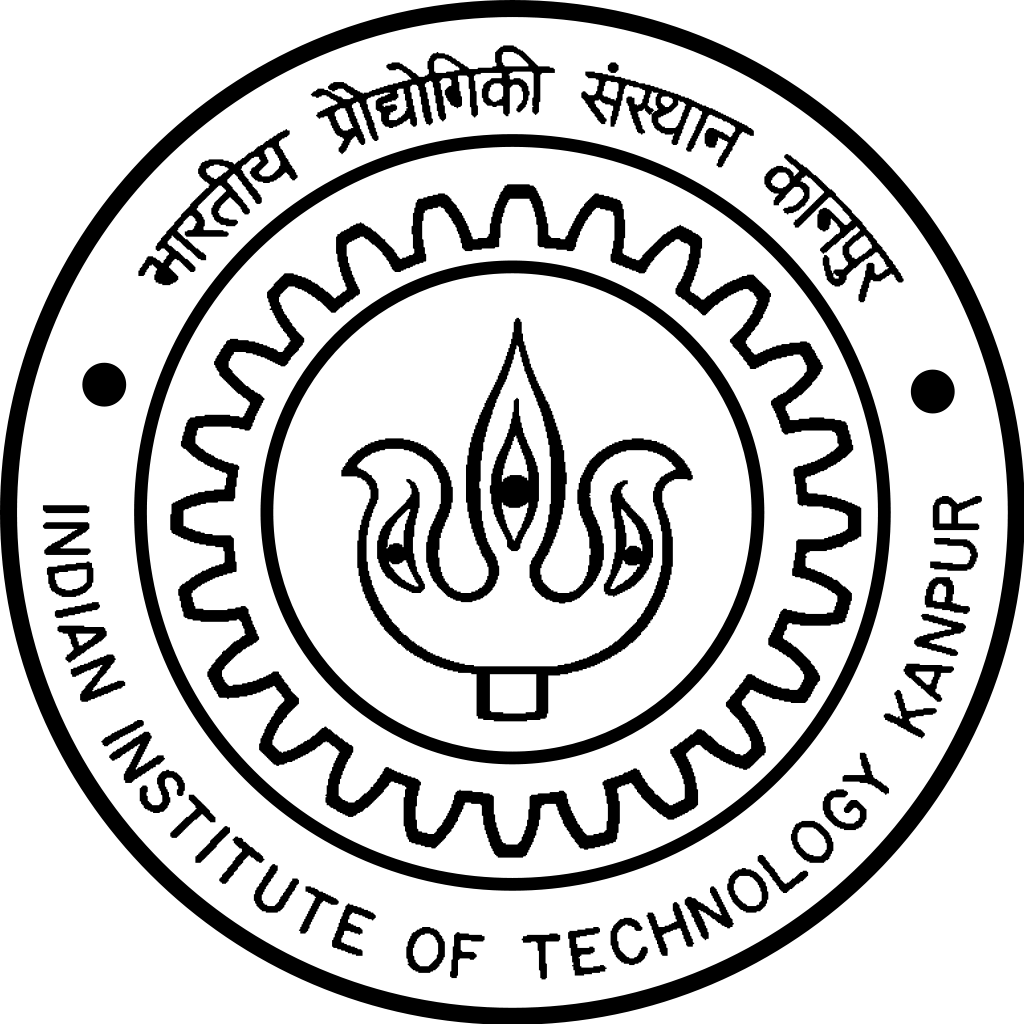
\includegraphics[width=0.25\textwidth]{iitklogo.png}
        
        \vspace{1\baselineskip}
        
        \uppercase{Department of Computer Science and Engineering\\
        \textbf{Indian Institute of Technology Kanpur}}\\
        
        \vspace{1\baselineskip}
        \textbf{June 2015}
        
    \end{center}
\end{titlepage}


%%-----------------------------------------------PAGE 2 Certificate

\frontmatter
\addcontentsline{toc}{chapter}{Certificate}
\begin{center}
\textbf{\Large{CERTIFICATE}}
\end{center}
\vspace*{3\baselineskip}
This is to certify that the work contained in this thesis entitled \textbf{\textit{"Inter-procedural analysis of Concolic Execution"}}, by \textbf{Ashwini Kshitij (Roll No. 10327165)}, has been carried out under my supervision and this work has not been submitted elsewhere for a degree.\\
\\[4\baselineskip]

  \small
  \vspace{2.0 cm}
  \begin{tabular*}{1.0\textwidth}{@{\extracolsep{\fill}} l r}
    \textbf{Dr. Subhajit Roy} 			 & 				\textbf{Dr. Amey Karkare}\\
    Assistant Professor,				 &				Assistant Professor,\\
    Department of CSE, 					 & 				Department of CSE,\\
    IIT Kanpur.							 &				IIT Kanpur.
    
  \end{tabular*}
\newpage


%%----------------------------------------------ABSTRACT
\addcontentsline{toc}{chapter}{Abstract}
\begin{center}
\textbf{\Large{ABSTRACT}}
\end{center}
\vspace {0.8 cm}

Interprocedural analysis is the cornerstone of determining precise program behavioral information. Using this technique we can avoid making overly conversative assumptions about the effects of procedures and the state at call sites. It aims at gathering informations across multiple procedures.  

\vspace {0.5 cm}

In this thesis, to extend the concept of concolic execution to interprocedural calls we instrument the function call site. For such instrumentation purposes we have used a tool called CIL. Just before the function call we set up the environment for calling the procedure which in turn enables it to follow through the concolic execution of parameters with the control flow from caller to callee. Similarly, just after the call instruction we restore the calling environment by restoring the symbolic values.

\vspace {0.5 cm}

Modifying the symbolic execution engine to collect the interprocedural analysis information can have widepread applications in software verification and testing. We can improve the coverage of test suites that are automatically generated by intraprocedural concolic executers.   

  






\newpage

%%----------------------------------------------ACKNOWLEDGMENT
\addcontentsline{toc}{chapter}{Acknowledgement}
\begin{center}
\textbf{\Large{Acknowledgements}}
\end{center}

\vspace{1.0 cm}

I acknowledge, with gratitude, my debt of thanks to Professor Subhajit Roy for his advise and encouragement and to Professor Amey Karkare for his aid and foresight. They presented me with the opportunity to tackle interesting problems in field of Software Testing. Their patient but firm guidance was critical to successful completion of my research.  

\vspace{0.5 cm}

I appreciate the support of my friends and wingmates who always provided me with the confidence and courage to tackle even the most challenging problems. Without their help and councel, the completion this work would have been immeasurably more difficult. 

\vspace{1.0 cm}

I also want to express my sincere gratitude to \textit {\textbf {BRNS}} for encouraging our research work. Their encouragement motivated me to follow through this project.

\begin{flushright}
\textbf{-Ashwini Kshitij}
\end{flushright}

\newpage

%%----------------------------------------------CONTENTS

\tableofcontents
\listoffigures
\listoftables


\mainmatter

%%---------------------------------------------CHAP 1 Intro

\chapter{Introduction}
%%\lhead{Chapter 1. \emph{Introduction}}


\hspace {0.4 cm}
Symbolic execution has been a recipient of significant attention during the past few years. It is now considered an effective technique in generation of high coverage test suites. The idea has been discovered around three decades ago but it was after significant improvements the potential of the idea was harnessed. One such important improvement was symbolic execution alongside keeping track of concrete values (concolic execution). The main advantage of this technique is that whenever constraint solving complications (like timeouts) occur during classical symbolic execution, it is alleviated using the concrete values.

All practical programs involve procedure calls. The symbolic execution is relatively simple if there are no function calls involved (\textit{intraprocedural analysis}). A function call tranfers the control from the caller to the callee. That function may very well modify the symbolic state of the variables. If we transition the symbolic state correctly through the function call, the symbolic execution will run correctly with the modified symbolic state and collect the precise alteration made to symbolic state within the procedure.    

%%----------------------------------------------MOTIVATION

\section{Motivation}
\textit{Intraprocedural Analysis} is performed on one procedure at a time. It is simple and conservative. But almost all real world programs involve procedural calls. This poses a problem for techniques such symbolic execution since they dont know how the procedure is going to modify the symbolic state. This brings us to the need of extending our analysis techniques to prgrams with functions and procedures.

%%----------------------------------------------PROBLEM STATEMENT

\section{Problem Statement}
This thesis aims to provide a method that can capture the transformation of the symbolic state of the inputs when the program goes through a function call. Our implementation uses inbuilt concolic execution engine for the purpose. But the engine cannot handle a procedure call. At the call site, the symbolic value is reset to "start state" instead of modifying it as per the operations performed on it by the callee function. Merging our approach with this concolic engine will increase the precision of test case generation. 

\begin{figure}[htbp]
\centering
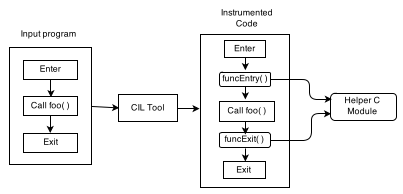
\includegraphics[scale=1]{module3.png}
\caption{Basic Module}
\end{figure}

\textit{Figure 1.1} shown above gives a high-level idea of what our implementation does. We are given a C program with a concolic execution engine integrated with it. Problem arises with execution when it comes across a procedure call instruction. The symbolic state of the input variables is set to default as the program does not have the ability to follow through symbolic execution from caller to callee and then back to the caller.

We aim at solving this problem by instrumenting the call site. For such purposes in our approach we have used a tool called CIL. We first set up an environment before commencing the callee procedure execution (in this case \textit{foo}). The operations for such tasks is carried out by \textit{funcEntry} function which is instrumented just before \textit{foo} is called. \textit{funcEntry} handles the mapping of symbolic and concolic values of actual parameters to formal parameters, the creation of symbolic stack (later explained in \textit{Chapter 3}).

Similarly we instrument \textit{funcExit} function just after \textit{foo} call. The task of \textit{funcExit} is to map the symbolic state of "return variable" to appropriate variable at the call site (if any) and clear the symbolic values that were generated during call and execution of \textit{foo}. It also manages the symbolic stack appropriately. The implementation of \textit{funcEntry} and \textit{funcExit} is done in C language and is defined in included C modules.

This approach ensures that symbolic execution is carried through correctly to and from the callee. The modified state of symbolic variables is in accordance with operations of concerned callee function (in our case \textit{foo}). This improves the accuracy and correctness of the test suite generation in our tool.  

%%----------------------------------------------CONTRIBUTIONS

\section {Contributions}
In this thesis we have accomplished the following:
\begin{itemize}
  \item Designed an approach to apply inter-procedural analysis to concolic execution. 
  \item Application of this technique to improve the automatic test case generation using concolic testing.
  \item Dynamic support to handle recursive procedure calls. 
\end{itemize}

%%----------------------------------------------ORGANISATION OF THESIS

\section {Organisation of thesis}
A brief summary of the contents of other chapters of this thesis are as follows.\\

\textbf{Chapter 2} deals with the concepts which are necessary to understand the thesis. Concolic execution is introduced and its advantages over classical symbolic execution and random testing. An overview of approaches in interprocedural analysis like Function Inlining and Call String have also been discussed in this chapter. We have also briefly mentioned the related work that has been done in this field. \\

\textbf{Chapter 3} discusses our implementation in a detailed manner. Some terminology has been introduced to explain techniques employed in our work. But mostly the chapter pertains to the relevant algorithms designed to accomplish the aim of this thesis and how it should improve the scalability and accuracy of concolic IP analysis.\\

\textbf{Chapter 4} contains the experimental results and their analysis after we run our modified tool on a set of standard benchmark programs. Analysis in done in terms of coverage improvement and runtime of the tool.\\

\textbf{Chapter 5} sheds light on future work and modifications that can be done to improve the accuracy and performance of the approach discussed in this thesis.

%%----------------------------------------------CHAPTER 2 : BACKGROUND

\newpage
\chapter{Background}

%%----------------------------------------------INTERPROCEDURAL DATAFLOW ANALYSIS

\section {Interprocedural Data-flow Analysis}
This is a technique which is broadly defined as gathering of information across multiple procedures (typically over the entire program). Procedure call poses barrier to program analysis. Its aim is to avoid making conservative assumpions about the effect of procedures and the state at call sites.

Interprocedural analysis is more demanding and challenging than intraprocedural analysis. Here we need to take into account the call-return and parameter passing mechanisms, local variable of the function and function recursion (can be unbounded). In some cases the called procedure is known only in run-time like with function pointers or with virtual functions. 

\textbf{Application :} Interprocedural analysis (IPA) enables the compiler to optimize the code across different files (whole-program analysis), and can result in significant performance improvements of the program by removing spurious data dependencies. Integrating IPA with intraprocedural concolic execution will help compute the precise behavior of function calls on the symbolic state of the variables.

%%----------------------------------------------FUNCTION INLINING 

\subsection {Function Inlining}
One of the approaches is \textit{function inlining} which is the simplest and most widely used approach for accurate interprocedural symbolic execution. We simply use the copy of procedure's Control Flow Graph (CFG) at each call site. This leads to function being re-analyzed at every call site. This is can be avoided using \textit{function summaries}. They are implemented by merging all states at the function exit after computing an intraprocedural path constraint in terms of function input.\\ 

\begin{figure}[htbp]
\centering
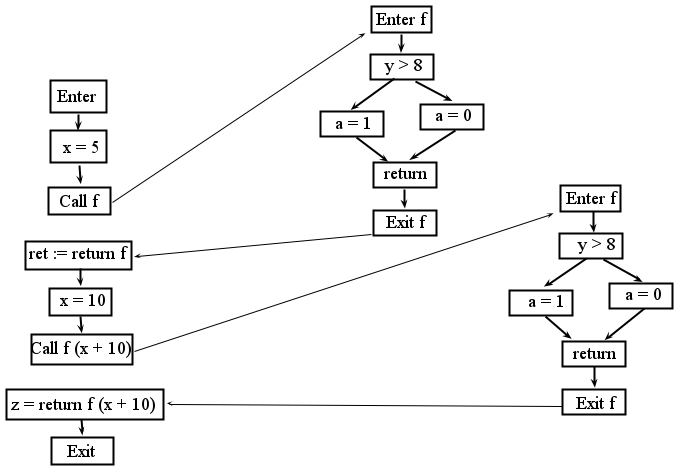
\includegraphics[scale=0.5]{inlineCFG.png}
\caption{Function Inlined}
\end{figure}

This technique does not require function calling overhead. It also saves the overhead for manipulating function stack. In increases locality of reference by utilizing instruction cache.

But there are significant \textit{drawbacks} with this approach. Firstly, the performance overhead will increase if we increase the size of the code that is to be inlined. The caller function may not fit on the cache causing high cache miss rate. Similarly if there are too many function calls involved, inlining maybe expensive since it will cause an exponential increase in the size of the CFG.

Secondly it is also going to create problems in the recursive procedures. Same can be said more generally for any scenario where there are cycles in the call graph. So basically function inlining has scalability issues pertaining to code size. Lastly, procedure inlining is only possible if the target of the call is known. Hence it will not be possible if call is via a pointer or is "virtual".

%%----------------------------------------------CALL STRING APPROACH

\subsection {Call String Approach}
In another IP analysis we observe the CFG's of all the procedures. In this technique,
\begin{itemize}
\item When we encouter a function call we interpret it as a goto from the call intruction to the first instruction of the procedure.
\item Interpreting every return statement like a goto to the instruction following each call site that invoked that procedure (\textit{Non-Deterministic}).
\end{itemize}
Using this method non-deterministically will allow non feasible paths in our analysis which will cause loss of accuracy. In a better approach called "Call String" we keep track of the where we came from, that is, the context of the call and where to return. To do this we maintain a "string" that simulates a call stack. A feasible path is a control flow path that is generated in accordance with the stack regime. A perfect solution is keep record of the whole stack. This concept is easy and intuitive according to which every return jumps to the instruction that's immediately after the call site which corresponds to that particular function call. By adding the context of the call to the information in the state we can overcome the problem of passing through invalid paths.\\

\begin{figure}[htbp]
\centering
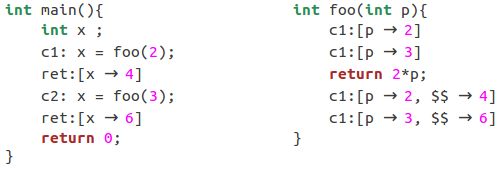
\includegraphics[scale=0.6]{callString.png}
\caption{Example : Call String}
\end{figure}  
 
Every procedure records their state information when they are invoked. Let us consider the program in \textit{Figure 2.2}. Here the labels \textit{c1} and \textit{c2} are saved in the state information of \textit{foo}. This is so that \textit{p} gets different values every time function \textit{foo} is called. Another reason to save the labels is because they help in figuring out the respective return values of call \textit{c1} (\$\$ $\rightarrow$ 4) and \textit{c2}(\$\$ $\rightarrow$ 6).

Implementing this algorithm is efficient for small strings. Problem arises when call string generated is large since we can keep track of only limited number of strings. This poses a limitation on the depth of function calls.

%%----------------------------------------------CONCOLIC TESTING


\section {Concolic Testing}

One popular approach for automated software testing is \textit{random testing} which involves subjecting the program to be tested to a stream of random data. It is fast but it can find only basic bugs like program crashes, code assertions or memory leaks. But it is not always possible to employ this technique specially when working with binaries since it is very difficult to figure out the expected inputs. The code coverage generated by random data is very low.\\

A more deliberate approach can be used by merging symbolic execution with concrete execution (\textit{concolic execution}) and then using a an SMT-solver (like Z3) to generate test inputs. This method is called \textit{Concolic testing}. It is much more efficient than symbolic execution. To understand why let us assume that our costraint solver cannot handle non-linear constraint. Then a path constraint with some \textit{non-linear} function involved cannot be solved and symbolic execution will be stuck. Similar problem arises when we encounter a closed third party library function say \textit{increment()}. Symbolic execution alogorithm doesn't know how to modify the symbolic state according to the behavior of that function. For such cases the test cases cannot be generated by classical symbolic execution. Concolic Tesing addresses these limitations and resolves situations like above by replacing the symbolic values by their concrete values so that the resulting constraint can be solved by the constraint solvers.\\

The algorithm involves initialting the inputs with randomly generated values. The program is executed and during the execution, on every conditional branch statement program collects symbolic path constraints on inputs. Symbolic constriants are essentially a set of logical constriants on input data. New program path is directed and executed by \textit{negating/flipping} the last condition of the path constraint. This is done until all the feasible program paths are explored. To get the intuition, let us consider the program in \textit{Figure 2.2} for concolic testing.  

\newpage

\begin{figure}[htbp]
\centering
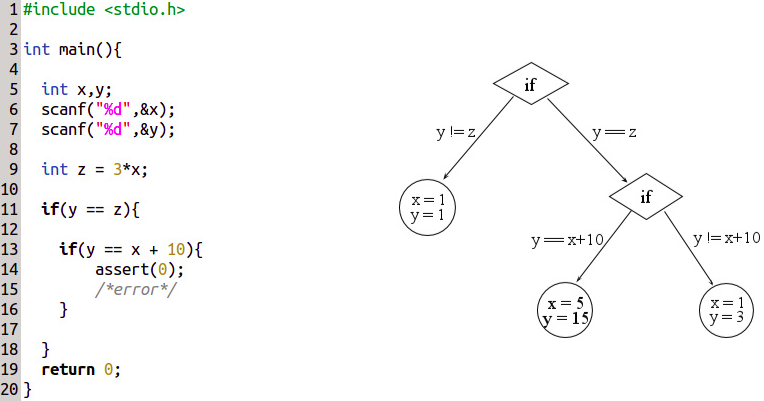
\includegraphics[scale=0.5]{conjoined4.png}
\caption{Concolic Testing}
\end{figure}

The program input variables are assigned random concrete values, say \textit{x = 1} and \textit{y = 1}. The program runs and line 11 is executed. Path condition generated is :

\begin{equation}
\neg(y == 3x)
\end{equation}

Now we negate the last condition in path constraint (PC has only one condition in this case) to execute an alternate path. So the new path constraint generated is :

\begin{equation}
y == 3x
\end{equation}

which is examined by a SMT solver to generate the new input data. Out of many different possible values for equation \textit{2.2} solver picks say \textit{x = 1} and \textit{y = 3} which should explore a different path than before. The program runs on these new inputs and generates a new path condition :

\begin{equation}
(y == 3x) \wedge \neg(y == x + 10)
\end{equation}

Like previously we negate the last condition of the path constraint to generate condition for new path exploration.
So we pass on the following constraint to solver to generate new inputs

\begin{equation}
(y == 3x) \wedge (y == x + 10)
\end{equation}

Let the new inputs generated be \textit{x = 5} and \textit{y = 15} we will lead to the execution of line 13 and consequently line 14 which will hit the error or any other unexpected behavior. Since there are no more paths left to explore, the algorithm will terminate generating a set of input data for complete path coverage of this program.

%%----------------------------------------------RELATED WORK

\section {Related work}

%%----------------------------------------------SUMMARY BASED ANALYSIS

\subsection {Summary-based Analysis}
New techniques have been invented that compute procedure summaries for performing an interprocedural analysis of programs. In summary-based context-sensitive analysis we create "summary" which is succinct description of the observable behavior of each procedure. The purpose of this approach is to prevent renanalysing the behavior of same procedure when there are invoked at each call site.

The representation of every procedure has a single entry point. The analysis is divided into following two phases:
\begin{itemize}
  \item In fist phase we summarize the effects of a procedure and a transfer function is computed in a bottom-up manner.
  \item  In second phase we propogate the caller information to compute callee result in a top-down manner.
\end{itemize}

%%----------------------------------------------DART

\subsection {DART}
DART is an abbreviation for "\textit{Directed Automated Random Testing}" which is a tool for automated test case generation developed by \textit{Patrice Godefroid, Nils Klarlund} and \textit{Koushik Sen}. It utilizes the concept of concolic execution and is comprised of the following techniques :
\begin{itemize}
 \item \textit{Automated} extraction of program interface from source code.
 \item \textit{Random testing} the program interface by generating a test driver. 
 \item Dynamic generation of test cases to \textit{direct} alternate program execution path.
\end{itemize}

\newpage

%%----------------------------------------------CUTE

\subsection{CUTE}
CUTE stands for "A Concolic Unit Testing Engine for C" which also addresses automatic test case generation with memory graphs as inputs. This tool is developed by \textit{Koushik Sen}, \textit{Darko Marinov} and \textit{Gul Agha}. It is similar to DART, thereby employs concolic testing technique. It resolves some of the limitations of DART and aims at testing real-world examples of C code.

It provides a method for representing and solving approximate pointer contraints to generate test inputs. The symbolic model being used is more powerful and the theorm solver is both more powerful and is built to be efficient in this system. As opposed to what DART does, CUTE does not automatically extract program interface but lets user decide relation among functions and their preconditions. The work also shows exactly how it made approximations and trade off between speed vs. correctness and scenarios where CUTE will not work correctly.






\newpage


\chapter{Methodology}
The algorithm that has been used to implement the interprocedural analysis in the concolic execution engine has been described in detail in this chapter.

\section{Definitions}

We are given a program \textbf{P} which has a concolic execution engine \textbf{C} integrated with it. Our aim is to combine interprocedural analysis with \textbf{P} so that the test case generation can also take into account the effect of function calls. To implement this algorithm we will instrument the code of P with our auxiliary code which will not alter the outcome of the program \textbf{P}. Let 

\begin{itemize}
 \item \textit{I} be the input generated by the tool for program P.
  \item \textit{\textbf{f}} be the callee function used in call site.
 \item \textit{Output(P,I)} be the output of the program P when run on input I. 
 \item \textit{\textbf{S}} denote Variable Stack explained in \textit{section 3.3.3}.  
\end{itemize}

\section{Static Analyser}
We have used a tool called \textbf{CIL} (\textbf{C} \textbf{I}ntermediate \textbf{L}anguage) to perform static analysis of program P and source-to-source transformations on it. We do this by tranversing the AST (Abstract Syntax Tree) which is the in-memory data-structure which represents the parsed program P.

\subsection{Handle Expressions}

This module accomplishes two tasks. It involves the simplification at call site with respect to the arguments (if any) passed to the function. It also simplifies the return expression at the end of function (if functions returns anything). 

At the call site the arguments of the function are examined one by one. If an argument is not a variable or literal then it must be an expression. In latter case, we store the argument in a temporary local variable and pass that new variable as the parameter instead. Similar approach applies to return values. If the return statement consists of a variable, it is left unchanged otherwise it is transformed.\\

\begin{figure}[htbp]
\centering
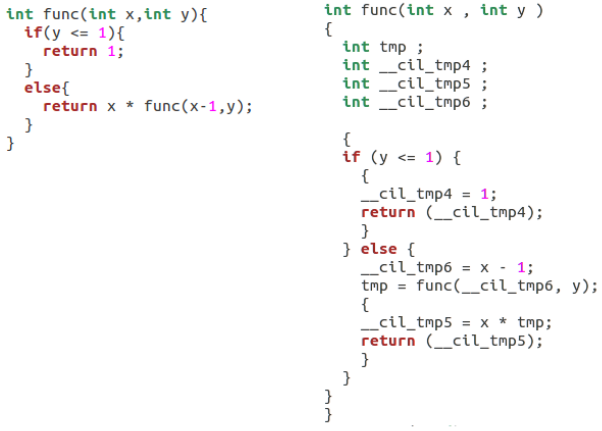
\includegraphics[scale=0.55]{handleExp3.png}
\caption{Original and Modified Function}
\end{figure}  

We can see in \textit{figure 3.1} the call sites and return statements have been transformed such that in further stages we only have to deal with variables. We will not have to deal with complicated expressions. To create new local temporary variable we use CIL API's. It ensures that the variable have unique names thus avoiding any ambiguity.
This phase will have no effect on function calls with no arguments or functions which don't return any value (void).
\newpage

\subsection{Variable Renaming}
The concolic testing engine we are using, uses a symbolic table structure that is globally defined, to carry out the symbolic execution. The entries in the table are manipulated using variable names of program P as the key. Until now the symbolic execution was intraprocedural, so we didn't have to deal with duplicate variable names.

But now we are dealing with multiple procedures and all of them will be capable of executing symbolically. Two different procedures may very well have variables with the same name. So when these variables are used as the key to manipulate the values in symbol table, the context of the variable will be ambiguous. This will cause undesired behavior in the concolic engine. 

Therefore we need to make the variables of all the procedures unique. This is done by renaming the variable in association with the name of the procedure in whose scope they belong. If \textit{K} is the key of the symbol table and \textit{V} be the variable name. Then before transformation, we have 

\begin{equation}
K = f(V)
\end{equation}

and after transformation we have

\begin{equation}
K = f(V,P)
\end{equation}

where \textit{P} is the name of the procedure to which V belongs. \textit{Figure 3.2} demonstrates the renaming of the variables to resolve the conflict of symbol table keys. This method will work for non-recursive procedure calls. To handle recursion we have developed an extended version of approach which will be discussed in \textit{section 3.4}.\\

\begin{figure}[htbp]
\centering
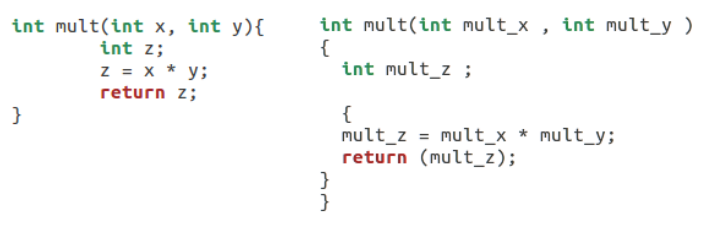
\includegraphics[scale=0.45]{renamed1.png}
\caption{Variable Renaming}
\end{figure}  

\newpage

\subsection{Extend Concolic Execution Engine}
The current engine uses approaches such as handling set (or assignment) instructions symbolically and unrolling of loops to carry out the symbolic execution. But these aproaches are only applied on the procedure that the user demands to be tested. The remaining procedures are unchanged.\\
Now on function call we want the symbolic execution to be able to continue in the callee \textit{f}. Hence we need to instrument all the procedures of program P such that it enables them to be executed symbolically. So instead of applying the loop unrolling and symbolic assignment only on user input procedure, they are applied on every procedure.

%%This can be understood using \textit{figure 3.4} which shows a function \textit{foo} which is not the function to be tested. Originally, \textit{foo} is unchanged since it plays no role in symbolic execution of program. Since we have want to extend the concolic engine to be executed interprocedurally, it is modified as shown. 

\subsection{Call Site Transformation}
Without interprocedural call handling whenever the concolic testing encountered a function call, it used the concrete value of the function result. There interprocedural symbolic analysis could not be done. This hindrance is removed by setting up a function call environment and function return environment, that will facilitate the transfer of symbolic state from caller to callee and back. The pseudo-code of the algorithm of this phase is mentioned on the next page.\\
\\
\textbf{Algorithm 1 Description} : The input to this algorithm is program P. We inspect all the procedures of P and detect the call sites. It is at these call sites where we need to do transformations such that when control flows from caller to callee, the callee has the symbolic information needed to execute symbolically.\\
Let one such call site be \textit{c} which invokes a function \textit{f}. Parameters that are passed to the function \textit{f} have certain symbolic and concrete values associated with them. Before \textit{f} starts executing, the mapping of concolic values needs to be done from actual parameters to formal parameters. For that we have to analyse the formal and actual parameters, and figure out a way to send their combined information to \textit{funcEntry}, which does the actual task of concolic mapping.\\ 
The function \textit{getArgumentsAsString} in \textit{line 8} has two parts. Firstly, it extracts the information about actual parameters of \textit{f} like if its a literal or variable (its name). Secondly, it analyses the formal parameters of \textit{f}'s prototype and gathers information about their name and type. Then it merges this information into a string, one parameter at a time.\\

\noindent\rule{15cm}{0.6pt} \\
 \textbf{\centerline{\textit{Algorithm 1: Transform Call Site}}}\\
\noindent\rule{15cm}{0.6pt} 

\noindent
\textbf{\textit{Input :}} Program P\\
\textbf{\textit{Output :}} P with modified call sites\\
\textbf{begin}\\
\linenumbers
\textbf{for} each procedure f $\in$ P \textbf{do}\\
\hspace*{2mm} InstList = instructionList(f)\\
\hspace*{3mm}\textbf{for} each instruction I' $\in$ InstList \textbf{do}\\
\hspace*{7mm}\textbf{if} I' is a Call Instruction C \textbf{then}\\
\hspace*{11mm}ArgsList = getArgumentsAsString(C $\rightarrow$ fname)\\
\hspace*{11mm}LocalsList = getLocalsAsString(C $\rightarrow$ fname)\\
\hspace*{11mm}FuncEntryInst = makeCallInstruction(ArgsList, LocalsList)\\
\hspace*{11mm}FuncExitInst = makeCallInstruction()\\
\hspace*{11mm}InstList = InstList :: [FuncEntryInst :: I' :: FuncExitInst]\\
\hspace*{7mm}\textbf{end if}\\
\hspace*{3mm}\textbf{end for}\\
\textbf{end for}\\
\textbf{end}

\nolinenumbers
\noindent

\vspace{0.4cm}
This string is passed as a paramter to \textit{funcEntry} along with another string containing the names of local variables (created by \textit{getLocalsAsString()} in \textit{line 9}). The function instrumented after call site \textit{c} is \textit{funcExit} that does the task of cleaning up the intermediate data-structures created by \textit{funcEntry} and were necessary to execute \textit{f} symbolically.

\begin{figure}[htbp]
\centering
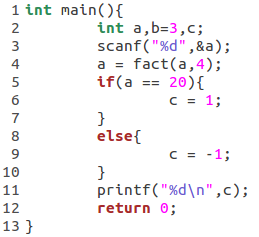
\includegraphics[scale=0.53]{env1_orig.png}
\caption{Original Code}
\end{figure}  

Let us observe an example shown in \textit{figure 3.4}. There is a call instruction at \textit{line 4} invoking function \textit{fact} with two paramters. The information about both actual and formal paramters in analysed and sent to \textit{funcEntry} as string argument at \textit{line 12} in \textit{figure 3.4}. The second argument to \textit{funcEntry} is names of local variables of function \textit{fact}. Using these arguments, environment for \textit{fact} to execute symbolically is set up by \textit{funcEntry}. Similarly, \textit{funcExit} at \textit{line 15 in figure 3.4} handles the task of cleanup of this environment after \textit{fact} has finished executing.

\vspace{0.4cm}
\begin{figure}[htbp]
\centering
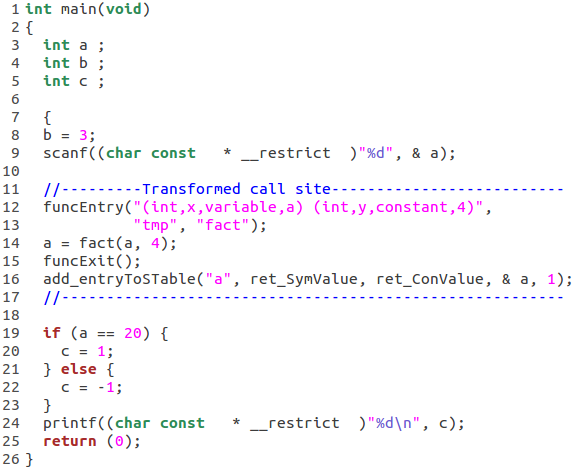
\includegraphics[scale=0.56]{env2_modified.png}
\caption{Transformed Call Site}
\end{figure}  

At \textit{line 16} in \textit{figure 3.4} we also have function \textit{add\_entryToSTable} which is used to map the returned concolic values of function \textit{fact} to appropriate variable, which is in our case \textit{a}. We will discuss about this in \textit{section 3.3.4}. 

\newpage

\section{Set up Environment For Procedure Call}
This section involves the runtime analysis of the arguments that are passed to \textit{funcEntry}. We will explain their utilization to create entries in global symbol table, to enable callee function \textit{f} to execute symbolically.

\subsection{Organising Argument Details}
Using the information of actual and formals parameters passed to the \textit{funcEntry}, we construct a data structure \textit{Argument} that has the following attributes: 
\begin{itemize}
 \item \textit{funcName} : name of the function to which the argument is passed.
 \item \textit{vname} : name of the associated formal parameter.
  \item \textit{type} : 1 for int and 2 for real.
 \item \textit{apname} : if actual argument is a variable, then its name.
  \item \textit{val} : if actual argument is a literal, then its value. 
\end{itemize}
Note that actual parameter can either be a variable or a literal, implying that only one among \textit{apname} or \textit{val} can have a valid value. The other is going to be \textit{null} so we have to use them accordingly. Recall that we have passed this parameter information along with local variable names of \textit{f} to \textit{funcEntry} as discussed in \textit{section 3.2.4}. Using string tokenizing and parsing within \textit{funcEntry}, we get a list of \textit{Arguments} type structures.\\
This step is demonstrated in \textit{figure 3.5} in reference to program shown in \textit{figure 3.4}.

\vspace{0.4cm}
\begin{figure}[htbp]
\centering
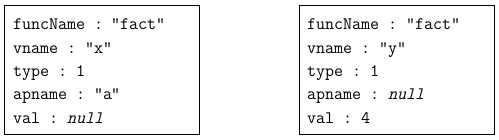
\includegraphics[scale=0.60]{arguments1.png}
\caption{Two arguments at \textit{line 12} in \textit{figure 3.4}}
\end{figure}

\newpage

\subsection{Populate Symbol Table}
After we created a systematic model of arguments, we need to populate the global symbol table accordingly. Besides the arguments, we also need to handle local variable in \textit{f}. For locals, we create empty entries in symbol table. The algorithm used in this implementation is described below


\noindent\rule{15cm}{0.6pt} \\
 \textbf{\centerline{\textit{Algorithm 2: Populate Symbol Table}}}\\
\noindent\rule{15cm}{0.6pt} 

\noindent
\textbf{\textit{Input :}} Argument list A, locals list L, symbol table S\\
\textbf{\textit{Output :}} Modified symbol table S' with entries for A and L\\
\textbf{begin}\\
\linenumbers[1]
\textbf{for} each argument a $\in$ A \textbf{do}\\
\hspace*{3mm}\textbf{if} a is a literal \textbf{then}\\
\hspace*{5mm}addEntryToSTable(a$\rightarrow$vname, "Constant", a$\rightarrow$val)\\
\hspace*{3mm}\textbf{else}\\
\hspace*{5mm}sym = findSymbolicValue(a$\rightarrow$apname)\\
\hspace*{5mm}con = findConcreteValue(a$\rightarrow$apname)\\
\hspace*{5mm}addEntryToSTable(a$\rightarrow$vname, sym, con)\\
\hspace*{3mm}\textbf{end if}\\
\textbf{end for}\\
\textbf{for} each local variable l $\in$ L \textbf{do}\\
\hspace*{3mm}createEmptyEntryInSTable(l$\rightarrow$name)\\
\textbf{end for}\\
\textbf{end}

\nolinenumbers
\vspace{6mm}
\noindent
\textbf{Algorithm 2 description} : This algorithm maps the symbolic and cocrete values of actuals parameters at call site to the formal parameters in the beginning of the function \textit{f}. For symbolic execution in \textit{f}, we also need to create initially empty entries of local variables in the table. Functions \textit{findSymbolicValue} and \textit{findConcreteValue} at \textit{line 8 and 9} search the symbolic and concrete values for a variable in the table. They are defined in the C modules of concolic testing engine.

\subsection{Variable Stack}
As we have seen in the previous section, before the execution of \textit{f} we have to populate symbol table with respective variables of \textit{f}. But same importance should be given to systematic clean up after \textit{f} is done executing, that is, deletion of entries from the table that were temporarily required for symbolic execution of \textit{f}. This is because these spurious values may not only cause inconsistencies but also caused the symbol table to overflow. 
For this purpose, we maintain a stack S called \textit{variable stack}. Each element of the stack stores the information regarding variable entries in the symbol table for indiviual function. The contents of stack element are as follows : 
\begin{itemize}
 \item \textit{funcName} : name of the function for which this element is created.
 \item \textit{args} : string array containing the names of formal paramters of \textit{funcName}.
  \item \textit{locals} : string array containing names of local variable in the scope of \textit{funcName}.
  \item \textit{occurence} : used to indicate the instance of \textit{funcName} in the call stack. We will explain this in detail and how it is used to resolve recursive calls in \textit{section 3.4.2}. 
\end{itemize}

\vspace{0.3cm}
\begin{figure}[htbp]
\centering
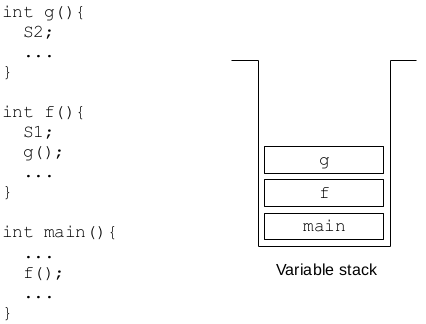
\includegraphics[scale=0.60]{stack.png}
\caption{Variable Stack}
\end{figure}

The behavior of variable stack is a lot alike to function call stack. Whenever we encounter a function call we push the variables (both arguments and locals) of the callee function onto the stack S. For example, in \textit{figure 3.6} when \textit{f} is called in \textit{main}, its variable details are pushed onto S. By the time statement S2 executes in \textit{g}, stack has three elements as shown in the figure.
When we return from a function call, we pop an element from the stack and delete the entries in the symbol table by referring the popped element.\\
The task of pushing the element on encountering a function call is done by a method \textit{funcEntry} and popping the element after returning from that function is done by \textit{funcExit}, both of which are defined in C modules.

\subsection{Return Handling}
After the environment is set up for \textit{f}, it executes symbolically covering some path in control flow graph of \textit{f}. It collects a summary that tranforms the symbolic values of parameters to new symbolic return values (if \textit{f} returns something). We need to map the concolic return values to appropriate variable at call site.\\ 
For this, just before the function \textit{f} returns, we copy the concolic return value to a global variable. Then at call site, we assign the lvalue of call instruction to this global concolic variable. Thus, the concolic execution flows to and from the callee correctly.   

\vspace{0.3cm}
\begin{figure}[htbp]
\centering
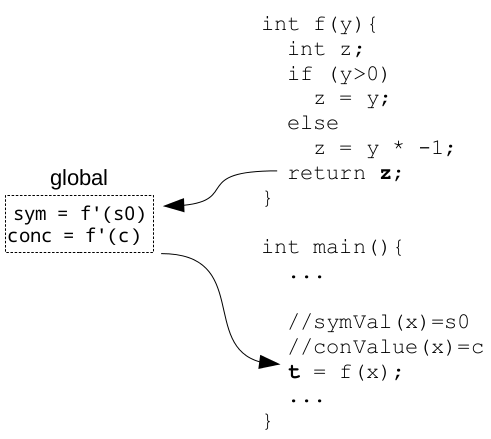
\includegraphics[scale=0.40]{return.png}
\caption{Concolic Return}
\end{figure}

Here in \textit{figure 3.7}, function \textit{f} is called with parameter x. Its symbolic and concrete value is modified according to function f', which is a transition function along some path in \textit{f}. Variable \textit{z} attains this new concolic value and is returned. To ensure transfer of modified symbolic information on function return, we map the concolic value of \textit{z} to global variable and from them to \textit{t} in \textit{main}, which is the intended recipient.

\newpage

\section{Recursion}
\subsection{Limitation of previous approach}
The approach that we have discussed until now can only handle non-recursive procedure calls. The reason being that our algorithm did not have support for multiple versions of same variable of the same function in the symbolic table. Our variable stack can handle atmost one instance of a function at any given time.
\{Recall that in \textit{section 3.2.2} we have resolved the issue of same named variables in different procedures.\}\\
To understand this, let us consider an example of recursive code.

\vspace{0.4cm}
\begin{figure}[htbp]
\centering
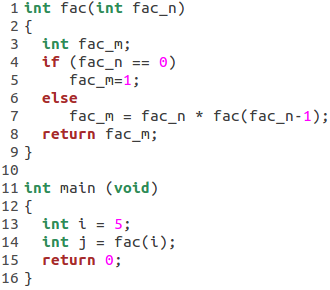
\includegraphics[scale=0.60]{fac.png}
\caption{WCET program for factorial}
\end{figure}

In this example, at \textit{line 14} a function call has been made to \textit{fac}. Before the call instruction executes, our algorithm maps concolic values from \textit{x} to \textit{fac\_n} and creates an entry in the symbol table using \textit{fac\_n} as the key. Now when the \textit{fac} executes, it again encounters a call instruction at \textit{line 7}. Our algorithm should map the values from \textit{fac\_n - 1} to "new" \textit{fac\_n}. But it has no mechanism implemented to distinguish between different versions of same variable of the same procedure. This leads to overwriting of previously present entry of \textit{fac\_n} in the symbol table (refer to \textit{table 3.1}) . More important problem that will arise is that after \textit{fact} at \textit{line 7} executes and returns, it cannot restore the previous symbolic state (i.e. before call was made). The concolic values of previous versions of the recurring function in the stack will be lost. \\
Therefore, we need to modify the key of symbol table such that we can keep track of multiple instances of same function in the variable stack, allowing recursive call analysis.



\begin{table}	
\begin{subtable}{.5\linewidth}
\centering
\begin{tabular}{||c c c||} 
 \hline
 \textbf{key} & \textbf{symVal} & \textbf{conVal} \\ [0.5ex] 
 \hline\hline
  & : &   \\ 
 %%\hline
  & : &  \\
 \hline
 fac\_n & s0 & c0 \\
 \hline
  & : &  \\ [1ex] 
 \hline
\end{tabular}
\caption{call at line 14}
\end{subtable}%
\begin{subtable}{.5\linewidth}
\centering
 \begin{tabular}{||c c c||} 
 \hline
 \textbf{key} & \textbf{symVal} & \textbf{conVal} \\ [0.5ex] 
 \hline\hline
   & : &   \\ 
  \hline
  fac\_n & s1 & c1 \\
  %%\hline
  \st{fac\_n} & \st{s0} & \st{c0} \\
  \hline
  & : &  \\ [1ex] 
 \hline
\end{tabular}
\caption{call at line 7}
\end{subtable}
\caption{Symbol Table} 
\end{table}

\subsection{Need for Versions}
We have to maintain versions of function variables according to number of instances they have in the variable stack. We have to make sure that the entries in the symbol table dont get deleted or overwritten unless they are not needed anymore. One way is to modify the keys (of symbol table) such that they have function version associated with them. \\
Let \textbf{occurence} of a procedure at any time be defined as the number of instances of that same procedure present in the call stack.\\

\vspace{0.4cm}
\begin{figure}[htbp]
\centering
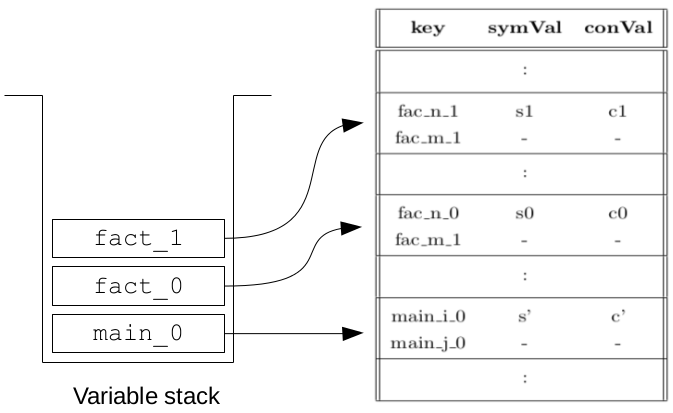
\includegraphics[scale=0.50]{symtableandstack.png}
\caption{Function Variable Versions in Symbol Table}
\end{figure}
Therefore we remodify the key defined in \textit{section 3.2.2} to keep track its associated variable, procedure to which that variable belongs and that procedure's version (\textit{occurence}) it the call stack. The new key is:

\begin{equation}
K' = f'(V,P,O_{\tiny{P}})
\end{equation}

where O$_{\tiny{P}}$ is the occurence of P in function call stack.
In \textit{figure 3.9} we can see the version handling of multiple instances of same functions in the symbol table. When another instance of function is pushed in the stack (recursively), no value in the symbol table is overwritten. Similarly, when a function instance is popped from the stack, the concolic values of previous version should be accessed.

\subsection{Variable Hash-Map}
The issue that arises with this approach is that we cannot rename variables in conjunction with their versions (like we did in \textit{section 3.2.2} using static analysis). This is because the versions are created dynamically at runtime when function call stack is manipulated. Therefore we create a hashmap \textit{M} that maps the variable name to key in the symbol table. At any point during execution, if procedure P is in the call stack, there will exist a mapping such that if K = f(V,P) then \textit{M} has following \textit{(key, value)} pairs

\begin{equation}
\textit{M} = (K,K')
\end{equation}

Whenever concolic execution needs to refer the symbol table using variable V, we look up the \textit{value} corresponding to V in \textit{M} and return the \textit{key}. But we still have to maintain the hashmap so that it always give the correct version of the key (the state of the variable stack is dynamic and so are the versions of function variables). To explain this let us consider a call instruction in the program that invokes function \textit{f}. The operations before and after the execution of \textit{f} are as follows.

\subsubsection{Before Function Execution}
In \textit{section 3.2.2} we discussed the algorithm to populate the symbol table with specific values before executing a call instruction. We modify that algorithm slightly, instead of using variable name K as key in \textit{addEntryToSTable}, we use our new key K'. Then we add the new mapping (K, K') to \textit{M}. This keeps track of key K' and its concolic values, for when we need to do a query on the symbol table.

\newpage
\subsubsection{After Function Execution}
When a function is done executing, the entries in the symbol table for that particular version of function are deleted. To do this, we again use the hashmap to get the current keys (containing current version of variables also) of symbol table that are no longer required.

\subsection{Bound on Recursion}
To keep the size of symbol table in check and prevent the variable stack from overflowing, we have to put an upper limit on the maximum number of instances that the variable stack can have of a given function. This puts a cap on the precision of symbolic execution. \\
If the maximum number of versions allowed for a particular function be \textit{C}, then the symbolic execution will only continue uptil stack depth of C, after that the function executes using only concrete values. The symbolic execution resumes when the stack depth with respect to that function becomes less than or equal to \textit{C}.









\chapter{Experiments}
\section{Result}
\section{Comparion of Test Case Generation}
\section{Analysis}

\chapter{Conclusion}
\newpage

\addcontentsline{toc}{chapter}{Bibliography}
\begin{center}
\textbf{\Large{Bibliography}}
\end{center}


\newpage
\vspace{0.5cm} 
\begin{tabular}{||c c c||} 
 \hline
 \textbf{key} & \textbf{symVal} & \textbf{conVal} \\ [0.5ex] 
 \hline\hline
   & : &   \\ [1ex]
  \hline
  fac\_n\_1 & s1 & c1 \\ [-1ex]
  fac\_m\_1 & - & - \\
  \hline
   & : &  \\ [1ex] 
  \hline
  fac\_n\_0 & s0 & c0 \\[-1ex]
  fac\_m\_1 & - & - \\
  \hline
  & : &  \\ [1ex] 
  \hline
  main\_i\_0 & s' & c' \\[-1ex]
  main\_j\_0 & - & - \\
  \hline
  & : &  \\ [1ex] 
 \hline
\end{tabular}
 


\end{document}
